\documentclass{beamer}
\usepackage[T2A]{fontenc}
\usepackage[utf8]{inputenc}
\usepackage[russian]{babel}
\usepackage{color}
\usepackage{hyperref}
\usepackage{listings}
\usepackage{color}
\usepackage{graphicx}
\usepackage{mathtools}
\usepackage{bm}
\usetheme{default}

\newcommand{\prevGender}{78,87\%}
\newcommand{\prevAge}{3,69}

\newcommand{\bestGender}{82,46\%}
\newcommand{\bestAge}{3,38}

\setbeamertemplate{footline}[frame number]

\title{Определение демографических характеристик пользователей
социальных сетей на основе анализа их музыкальных интересов}
\author{\textbf{Семёнов~A.~C.,} \\ 
    магистрант кафедры КТ университета ИТМО, \\
    semkagtn@gmail.com}
\institute{СПИСОК 2016}
\date{\today}

\subject{Научно-исследовательская работа}

\begin{document}

\begin{frame}
  \titlepage
\end{frame}

\begin{frame}{Интернет и его пользователи}
  \begin{itemize}
      \item {Огромное число пользователей}
          \begin{itemize}
              \item {Facebook~--- $968 \cdot 10^{6}$ уникальных посещений сайта в день}
              \item {Vkontakte~--- $75 \cdot 10^{6}$ уникальных посещений сайта в день}
              \item {Instagram~--- $400 \cdot 10^{6}$ уникальных посещений сайта в месяц}
          \end{itemize}
      \item {Информация о пользователях находится в открытом доступе}
          \begin{itemize}
              \item {Текст, который пишут пользователи}
              \item {Фотографии пользователей}
              \item {Интересы: фильмы, музыка, хобби}
              \item {Страна, город, геолокация}
              \item {Пол, возраст}
              \item {И т.д}
          \end{itemize}
  \end{itemize}
\end{frame}

\begin{frame}{Задача профилирования пользователей}
  \begin{itemize}
      \item {Информация о пользователях часто является неполной или отсутствует}
      \item {Задача: определить отсутствующие характеристики по имеющимся (по музыке)}
      \item {Характеристики пользователей являются ключевыми признаками в рекомендательных системах}
      \item {Существует множество подходов к определению характеристик пользователей}
          \begin{itemize}
              \item {Информация о музыке пользователей используется не часто}
              \item {Метод, использующий музыкальные предпочтения, может помочь улучшить существующие алгоритмы}
          \end{itemize}
  \end{itemize}
\end{frame}

\begin{frame}{Источник данных~--- Last.fm}
    \begin{figure}
        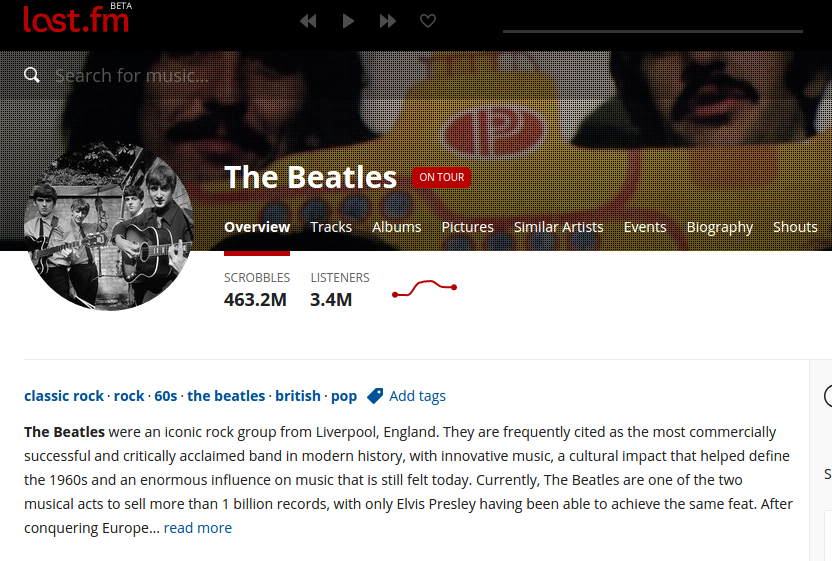
\includegraphics[width=\textwidth]{figures/lastfm.png}
    \end{figure}
\end{frame}

\begin{frame}{Задача определения характеристик пользователей}
    \begin{figure}
        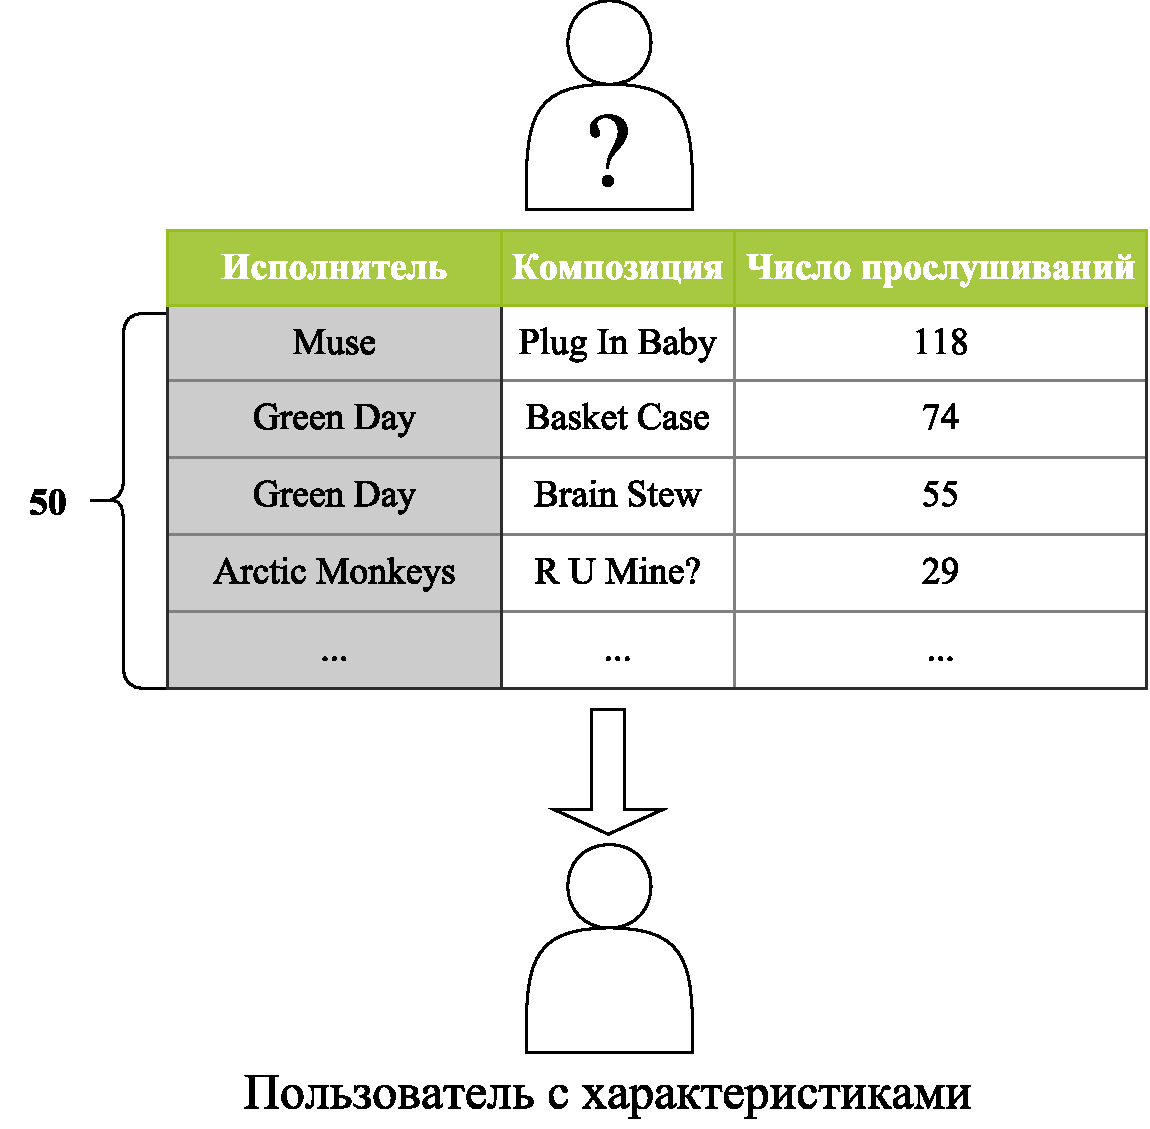
\includegraphics[scale=0.40]{figures/lastfm-top.pdf}
    \end{figure}
\end{frame}

\begin{frame}{Матрица исполнитель--пользователь}
  \begin{itemize}
      \item {Пользователи~--- документы, исполнители~--- термины}
      \item {$D = \{d_{ij}\}$~--- матрица термин--документ}
      \item {$d_{ij} = \mathrm{tf}_{ij} \cdot \log{\frac{n}{\mathrm{df}_{i}}}$ (Формула TF-IDF)}
          \begin{itemize}
              \item $\mathrm{tf}_{ij}$~--- число встреч термина $i$ в документе $j$
              \item $\mathrm{df}_{i}$~--- число документов, в которых встречается термин $i$
              \item $n$~--- общее число документов
          \end{itemize}
      \item {$d_{ij} = \begin{cases}
          0,& \mathrm{tf}_{ij} = 0,\\
          l(\mathrm{tf}_{ij}) \cdot g(\frac{n}{\mathrm{df}_{i}}),& \mathrm{tf}_{ij} \ne 0
      \end{cases}$}
          \begin{itemize}
              \item {$l(x), g(x)$~--- неубывающие неотрицательные функции}
          \end{itemize}
  \end{itemize}
\end{frame}

\begin{frame}{Латентный семантический анализ}
  \begin{itemize}
      \item {Каждый пользователь описывается вектором-столбоцом матрицы $D$}
      \item {Размерность векторов оказывается большой}
      \item {Используя метод \textit{LSI}, можно уменьшить размерность векторов (например, до $200$)}
      \item {Каждый пользователь описан числовым вектром размерности $200$}
  \end{itemize}
\end{frame}

\begin{frame}{Подход на основе Word2Vec}
  \begin{itemize}
      \item {Пользователи~--- предложения, исполнители~--- термины}
      \item {\textit{Word2Vec} преобразует термины в вектора произвольной размерности (например, $200$)}
      \item {$\bm{d}_{i} = \sum\limits_{n}{f(n) \cdot \bm{w}_{in}}$}
          \begin{itemize}
              \item {$\bm{d}_{i}$~--- вектор пользователя}
              \item {$\bm{w}_{in}$~--- исполнитель пользователя $i$, находящийся на позиции $n$}
              \item {$f(n)$~--- невозрастающая неотрицательная функция на отрезке $[1; 50]$}
          \end{itemize}
      \item {Каждый пользователь описан числовым вектром размерности $200$}
  \end{itemize}
\end{frame}

\begin{frame}{Модель на примере определения пола и возраста}
    \begin{itemize}
        \item {Использовался набор данных из существующего 
              исследования~\footnote{Wu M. J.,
              Jang J. S. R., Lu C. H. Gender Identification
              and Age Estimation of Users Based on Music 
              Metadata // The International Society of Music Information Retrieval (ISMIR). – 2014. – P.~555--560.}}
        \item {Всего $96807$ пользователей}
            \begin{itemize}
                \item {48404 пользователей в обучающей выборке}
                \item {48403 пользователей в контрольной выборке}
            \end{itemize}
        \item {У каждого пользователя указан пол и возраст}
        \item {Пользователь описан исполнителями из top-50 наиболее
            прослушиваемых им композиций}
        \item {Особенности выборки}
            \begin{itemize}
                \item {66{,}2\% и 33{,}8\% мужчин и женщин соответственно}
                \item {Возраст пользователей смещён в сторону молодого поколения}
            \end{itemize}
    \end{itemize}
\end{frame}

\begin{frame}{Обучение классификатора/регрессора}
  \begin{itemize}
      \item {Определение пола~--- задача бинарной классификации}
          \begin{itemize}
              \item {Качество~--- точность}
          \end{itemize}
      \item {Определение возраста~--- задача восстановления регрессии}
          \begin{itemize}
              \item {Качество~--- средняя абсолютная ошибка}
          \end{itemize}
      \item {Метод опорных векторов с ядром \textit{RBF}}
      \item {Параметры $C$ и $\gamma$ настраивались методом \textit{Grid Search Cross Validation} на обучающей выборке}
      \item {Векторы пользователей были нормализованы перед использованием метода опорных векторов}
  \end{itemize}
\end{frame}

\begin{frame}{Результаты: матрица исполнитель--пользователь}
    \[d_{ij} = \begin{cases}
              0,& \mathrm{tf}_{ij} = 0,\\
              l(\mathrm{tf}_{ij}) \cdot g(\frac{n}{\mathrm{df}_{i}}),& \mathrm{tf}_{ij} \ne 0
        \end{cases}\]
    \begin{table}[h!]
    \centering
    \begin{tabular}{|c|c|c|c|}
    \hline
    \boldmath$l(x)$ & \boldmath$g(x)$ & \textbf{Определение пола} & \textbf{Определение возраста} \tabularnewline
    \hline
    $1$ & $1$ & \textbf{82,46\%} & \textbf{3,54} \tabularnewline
    \hline
    $\log{x}$ & $1$ & 81,58\% & 3,64 \tabularnewline
    \hline
    $\log{x}$ & $\log{x}$ & 81,67\% & 3,57 \tabularnewline
    \hline
    $\log{x}$ & $\sqrt{x}$ & 80,04\% & 3,76 \tabularnewline
    \hline
    $\sqrt{x}$ & $1$ & 81,73\% & 3,63 \tabularnewline
    \hline
    $\sqrt{x}$ & $\log{x}$ & 81,76\% & 3,57 \tabularnewline
    \hline
    $\sqrt{x}$ & $\sqrt{x}$ & 79,78\% & 3,77 \tabularnewline
    \hline
    $x$ & $1$ & 79,45\% & 3,92 \tabularnewline
    \hline
    $x$ & $\log{x}$ & 79,67\% & 3,85 \tabularnewline
    \hline
    $x$ & $\sqrt{x}$ & 78,75\% & 3,88 \tabularnewline
    \hline
    \end{tabular}
    \label{tab:tfidf_results}
    \end{table}
\end{frame}

\begin{frame}{Результаты: модель Word2Vec}
    \[d_{i} = \sum_{n}{f(n) \cdot w_{in}}\]
    \begin{table}[h!]
    \centering
    \begin{tabular}{|c|c|c|}
    \hline
    \boldmath$f(n)$ & \textbf{Опредление пола} & \textbf{Определение возраста} \tabularnewline
    \hline
    $1$ & 78,12\% & 3,97 \tabularnewline
    \hline
    $\frac{1}{\log{n + 1}}$ & 79,61\% & 3,59 \tabularnewline
    \hline
    $\frac{1}{n^2}$ & 78,66\% & 4,02 \tabularnewline
    \hline
    $\frac{1}{n}$ & 80,22\% & 3,75 \tabularnewline
    \hline
    $\frac{1}{\sqrt{n}}$ & \textbf{81,46\%} & \textbf{3,38} \tabularnewline
    \hline
    $51 - n$ & 77,85\% & 4,03 \tabularnewline
    \hline
    $\log{51} - \log{n}$ & 78,16\% & 3,95 \tabularnewline
    \hline
    $\sqrt{51} - \sqrt{n}$ & 78,12\% & 3,98 \tabularnewline
    \hline
    \end{tabular}
    \label{tab:doc2vec_results}
    \end{table}
\end{frame}

\begin{frame}{Результаты: сравнение с достигнутыми ранее}
    \textit{best}~--- результаты текущего исследования \\
    \textit{baseline}~--- Wu M. J.,
        Jang J. S. R., Lu C. H. Gender Identification
        and Age Estimation of Users Based on Music 
        Metadata // The International Society of Music Information Retrieval (ISMIR). – 2014. – P.~555--560.
    \begin{table}[h!]
    \centering
    \begin{tabular}{|c|c|c|}
    \hline
    \textbf{Тип задачи} & \textbf{best} & \textbf{baseline} \tabularnewline
    \hline
    Определение пола & \textbf{\bestGender} & \prevGender \tabularnewline
    \hline
    Определение возраста & \textbf{\bestAge} & \prevAge \tabularnewline
    \hline
    \end{tabular}
    \label{tab:total_results}
    \end{table}
\end{frame}

\begin{frame}
    \titlepage
\end{frame}



\end{document}
